%!TEX root = ../../root.tex

Computer vision has been one of the first applications of rudimentary GDL. Let's see some proposed solutions to problems dealing with meshes.

What is a mesh? In practice, when we deal with manifolds, we deal with discrete representations of them. One possible way to represent a surface is using a graph (we have a sampling of the vertices and then we connect neighboring vertices using edges). However, a surface has no ``holes'' between its vertices, but instead the edges are ``filled'', with a \emph{face}. So, when we know that we are dealing with a surface that represents a real object, like a horse, we use a structure called \emph{mesh} which is a collection of polygonal faces where we have vertices, edges and also we have faces. We want to have some constraints on the faces, and these constraints make up what is called manifold mesh.
\begin{figure}[H]
	\centering
	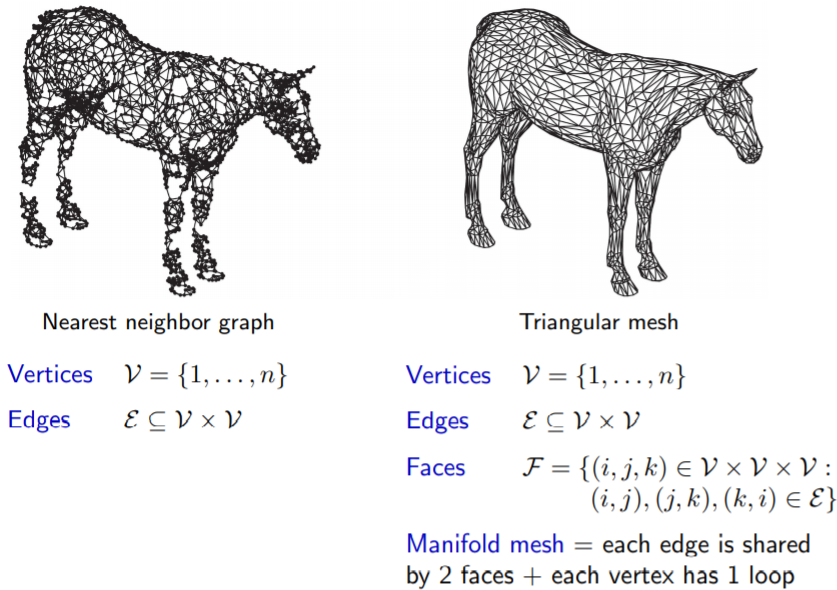
\includegraphics[width=.7\textwidth]{12/15_46}
	\caption{Discrete manifold.}\label{fig:disc-manifold}	
\end{figure}

\paragraph{Multi-view CNN}
Suppose we are given a dataset of $3D$ objects, and we want to classify them, e.g. to recognize furniture like tables, chairs and so on.

One approach that has been proposed to the task is called \emph{multi-view CNN}. The idea is that we can treat the data as a collection of $2$D images obtained just going around each object and taking a snapshot. Now, we can consider these images as items in our familiar Euclidean domain, and for instance employ the usual CNNs. However, since the images of an object all represent the same object, the networks should have some form of weight sharing, and at the end we would want to combine the prediction from each network in some way, for example using some kind of pooling.
\begin{figure}[H]
	\centering
	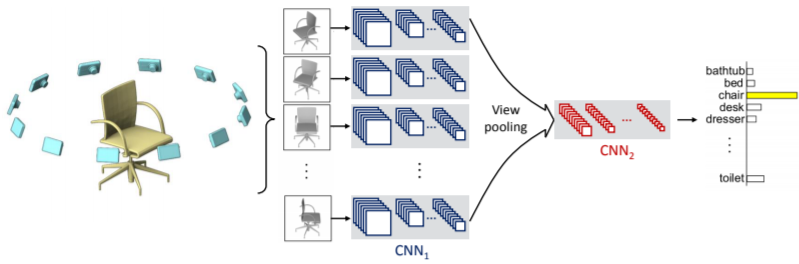
\includegraphics[width=.9\textwidth]{12/8_46}
	\caption{Multi-view CNN.}\label{fig:multi-viewCNN}	
\end{figure}
Other applications of this approach, in addition to the classification of $3$D objects, are sketch classification (training the model with a different rendering) and sketch-based shape retrieval (rendering the different views of the objects).
\begin{figure}[H]
	\centering
	\begin{subfigure}[t]{0.3\linewidth}
		\centering
		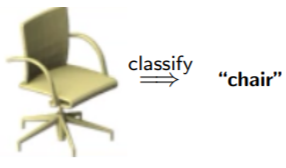
\includegraphics[width=\textwidth]{12/9_46_a}
		\caption{3D shape classification and retrieval.}
	\end{subfigure}
	\hfill
	\begin{subfigure}[t]{0.3\linewidth}
		\centering
		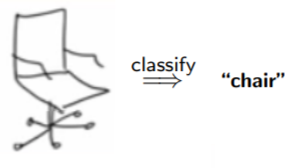
\includegraphics[width=\textwidth]{12/9_46_b}
		\caption{Sketch classification.}
	\end{subfigure}
	\hfill
	\begin{subfigure}[t]{0.3\linewidth}
		\centering
		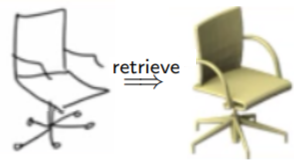
\includegraphics[width=\textwidth]{12/9_46_c}
		\caption{Sketch-based shape retrieval.}
	\end{subfigure}
	\caption{Application of multi-view CNN.}\label{fig:app-multiviewCNN}
\end{figure}
Note that this approach is not invariant to rotations in space, so it works well only if the object is rigid.

\paragraph{$3$D ShapeNets}
Another idea is representing a $3$D object using \emph{voxelization}, \textit{i.e.} represent it as a collection of small $3$D cubes, named \emph{voxel}, the $3D$ counterpart of the $2D$ \emph{pixel}. In this setting we can define a standard $3$D convolution. Note that we are not looking at the surface but at the interior of the surface.
\begin{figure}[H]
	\centering
	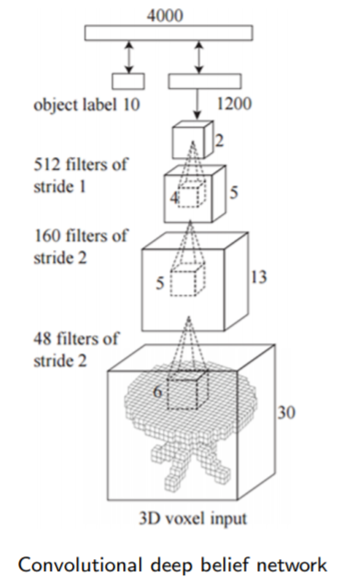
\includegraphics[width=.4\textwidth]{12/10_46}
	\caption{$3$D ShapeNet.}\label{fig:3d-shapenet}	
\end{figure}

Using $3$D shape nets, just like in $2$D neural network, we can learn hidden features, which we call $3$D primitives, that are organized in a hierarchical fashion as we go deeper and deeper into the network, recognizing semantically valid features at the deepest level.
\begin{figure}[H]
	\centering
	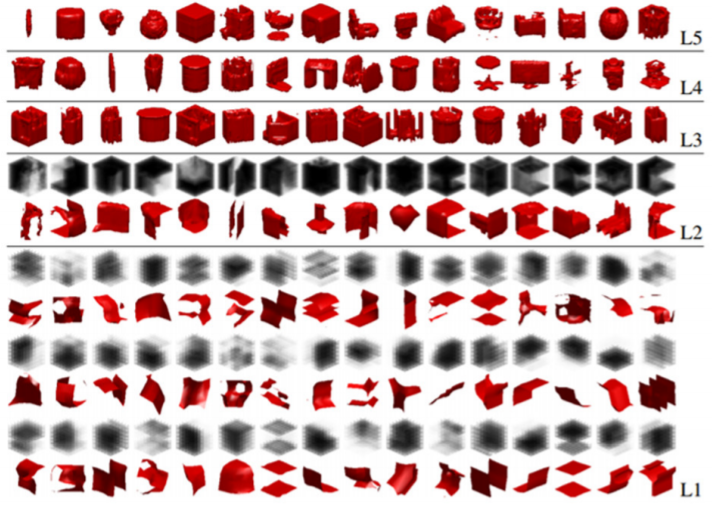
\includegraphics[width=.6\textwidth]{12/11_46}
	\caption{$3$D primitives}\label{fig:primitives}	
\end{figure}

% To obtain deformation invariants we want that the filters in our $3$D convolution operate directly on the top of the surface, so when the object bends also the filter bends with the object and whatever we learn on the original object is also valid for the deformed object.
% \begin{figure}[H]
% 	\centering
% 	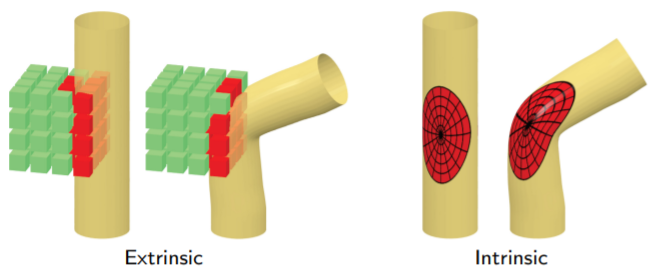
\includegraphics[width=.8\textwidth]{12/12_46}
% 	\caption{Extrinsic vs Intrinsic}\label{fig:deformations}	
% \end{figure}

% Unlike images, there is no canonical ordering of the domain points in graphs and meshes. This is relevant, since we want to define something close to convolution and it involves the concept of neighborhood in according to the size of convolutional filter, and the absence of this concept is a critical issue, named local ambiguity; for instance in a graph if we are given a node and we want to access to its neighbors there is no canonical way of visiting the neighbors, while for meshes we have a notion of orientation \textit{i.e.} label the neighbors of a node in a clockwise sense but fix the first one remain ambiguous.
% \begin{figure}[H]
% 	\centering
% 	\includegraphics[width=.9\textwidth]{12/16_46}
% 	\caption{Local ambiguity.}\label{fig:loc-amb}	
% \end{figure}